\documentclass[paper=a4,headings=small,titlepage,makeidx,fontsize=12pt]{scrbook} 

% ===========================================================================
% PREAMBLE
% ===========================================================================
% ===========================================================================
% PREAMBLE STANDARD (English)
% ===========================================================================
\usepackage{fontspec}%           provides font selecting commands
\usepackage{xunicode}%           provides unicode character macros
\usepackage{xltxtra} %           provides some fixes/extras
%\usepackage[utf8x]{inputenc} %  problems with xetex?
%\usepackage[utf8]{inputenc} %   problems with xetex?
%\usepackage[T1]{fontenc} %      problems with xetex and UF8?
\usepackage{tabularx}%           order matters
\usepackage{tikz}%               order matters
%\usepackage{pgf-pie} %          order matters
\usepackage{wallpaper} %         order matters
\usepackage{tabu} %              make thick lines
\usepackage{colortbl} %          make color lines
\usepackage[]{graphicx}
\usepackage{xcolor}
\usepackage{hyperref}%           configured later!
\usepackage{fullpage,longtable}% better tables
\usepackage{hhline}%             better tables
\setlength{\parindent}{0cm}
\setlength{\arrayrulewidth}{2pt}

% ===========================================================================
% SET FONTS 
%\usepackage{pifont}
%\usepackage{helvet}
\usepackage{latexsym}
\usepackage{amssymb,amsmath}

%\setmainfont{Ume Mincho S3}    % Serif      2 OK
%\setmainfont{AR PL UMing HK}   % Typewriter 1 GOOD
%\setmainfont{Sawarabi Gothic}   % SanSerif   1 GOOD
%\setmainfont{WenQuanYi Zen Hei}% SanSerif   2 OK (wrong g?)
%\setmainfont{Komatuna P}       % SanSerif   3 MAMA (but strong!)

% Should be LMRoman12 though
%\setmainfont[Mapping=tex-text]{LMRoman10}
%\setsansfont{AR PL UMing HK}
%\setmonofont{AR PL UMing HK}

%\setmainfont{IPAPMincho}
%\setmonofont{IPAPGothic}
%\setsansfont{IPAPMincho}
%\setmainfont{IPAPMincho}
%\setmonofont{IPAMincho}
%\setsansfont{IPAPMincho}

%\fontspec[
%ItalicFont={IPAGothic},
%BoldFont={IPAGothic},
%ItalicFeatures={FakeSlant},
%BoldFeatures={FakeBold=1.5},
%]{IPAPMincho}

%BoldFont = URW Palladio L, 
%ItalicFont = URW Palladio L,
%BoldItalicFont = URW Palladio L,
%SlantedFont = URW Palladio L,
%BoldSlantedFont = URW Palladio L,
%SmallCapsFont = URW Palladio L,
%UprightFont = *-Roman
%\setmainfont{YOzFontE}   % SanSerif   1 GOOD
%\setmonofont{AR PL UMing HK}

\defaultfontfeatures{Ligatures=TeX}
\setmainfont[SlantedFont={LMRoman10},
             SlantedFeatures={FakeSlant=0.2}]{LMRoman10}
\setsansfont[SlantedFont={LMRoman10},
             SlantedFeatures={FakeSlant=0.2}]{LMRoman10}

\usepackage{array}% for vertical alignment in tabular with m{SIZE}
\usepackage{xeCJK}
\usepackage{ruby}
\renewcommand{\rubysep}{0.25ex}
\setCJKmainfont{IPAPMincho}
\setCJKfamilyfont{JapaneseDejima}{Dejima}
\setCJKfamilyfont{JapaneseYOzFont}{YOzFont90} %hand
\setCJKfamilyfont{JapaneseYOzFontA}{YOzFontA}
\setCJKfamilyfont{JapaneseYOzFontC}{YOzFontC90}
\setCJKfamilyfont{JapaneseYOzFontE}{YOzFontE90}
\setCJKfamilyfont{JapaneseYOzFontF}{YOzFontF90}
\setCJKfamilyfont{JapaneseYOzFontM}{YOzFontN90}
\setCJKfamilyfont{JapaneseYOzFontP}{YOzFontP90}
\setCJKfamilyfont{JapaneseIPAPGothic}{IPAPGothic}
\setCJKfamilyfont{JapaneseDefault}{IPAPMincho}
\newcommand\JapaneseYOzFont{\CJKfamily{JapaneseYOzFont}\CJKnospace}
\newcommand\JapaneseYOzFontA{\CJKfamily{JapaneseYOzFontA}\CJKnospace}
\newcommand\JapaneseYOzFontC{\CJKfamily{JapaneseYOzFontC}\CJKnospace}
\newcommand\JapaneseYOzFontE{\CJKfamily{JapaneseYOzFontE}\CJKnospace}
\newcommand\JapaneseYOzFontF{\CJKfamily{JapaneseYOzFontF}\CJKnospace}
\newcommand\JapaneseYOzFontM{\CJKfamily{JapaneseYOzFontM}\CJKnospace}
\newcommand\JapaneseYOzFontP{\CJKfamily{JapaneseYOzFontP}\CJKnospace}
\newcommand\JapaneseIPAPGothic{\CJKfamily{JapaneseIPAPGothic}\CJKnospace}
\newcommand\JapaneseIPAPMincho{\CJKfamily{JapaneseIPAPMincho}\CJKnospace}
\newcommand\JapaneseGothic{\CJKfamily{JapaneseIPAPGothic}\CJKnospace}
\newcommand\JapaneseDejima{\CJKfamily{JapaneseDejima}\CJKnospace}
\newcommand\JapaneseDefault{\CJKfamily{JapaneseDefault}\CJKnospace}

%\setCJKsansfont[]{}
%\setCJKmonofont[...]{...}

% Should be LMRoman12 though
%\newcommand{\Circ}[1]{\fontspec{Sawarabi Gothic}#1\setmainfont{LMRoman10}}

% ===========================================================================
% WRITE JAPANESE TEXT VERTICALLY
% derived from jltxdoc.cls and plext.dtx
%\usepackage{plext}
\def\tsample#1{%
%  \hbox to\linewidth\bgroup\vrule width.1pt\hss
  \hbox to 150mm \bgroup\vrule width.1pt\hss
    \vbox\bgroup\hrule height.1pt
      \vskip.5\baselineskip
%      \vbox to\linewidth\bgroup\tate\hsize=#1\relax\vss}
      \vbox to 150mm \bgroup\tate\hsize=#1\relax\vss}
\def\endtsample{%
      \vss\egroup
      \vskip.5\baselineskip
    \hrule height.1pt\egroup
  \hss\vrule width.1pt\egroup}

% ---------------------------------------------------------------------------
% ADD THIS PACKAGES INCASE latex AND NOT platex is used:
% \documentclass[titlepage,12pt,a4paper,german]{book}
% PAKETE
% Deutsche Umlaute etc.
% \usepackage{2up}
% \usepackage{natbib}
% \bibpunct[;]{(}{)}{;}{a}{,}{,}
% Sprache (nach natbib)
% \usepackage{babel}
% pakete aus deutscher distribution
% \usepackage{2up}


% ===========================================================================
% Better hypphenation - more space
\sloppy
\hyphenation{
bei-spiels-wei-se
chi-nesi-sche 
chi-nesi-sch-en
ein-ge-se-tzt
Ge-sell-schafts-ge-spra-che
gram-mati-schen
Ja-pa-ni-sch 
Kanji-Kana-Majiri-Bun 
Schrei-bung 
Schrift-sys-tem
Schrift-zei-chen 
}


% ===========================================================================
% PAGELAYOUT
\usepackage{geometry}
\geometry{
  top=1in,            % <-- you want to adjust this 0.5
  inner=.8in,
  outer=.6in,
  bottom=1.5in,
  footskip=5ex,   
  headheight=5ex,       % <-- and this 3
  headsep=5ex,          % <-- and this 2
}
% better head lines
\usepackage{fancyhdr}
\pagestyle{fancy}
%\fancyhead{30pt}
\setlength\headheight{25.5pt}


% ===========================================================================
% NEW DEFINITIONS FOR SYSTEM COMMANDS
\renewcommand{\chaptermark}[1]{\markboth{\textsf{\scriptsize \thechapter.\ #1\normalsize}}{}}
\renewcommand{\sectionmark}[1]{\markright{\textsf{\scriptsize\thesection.\ #1\normalsize}}{}}
 
%\renewcommand{\chaptermark}[1]{%
%\markboth{\textsf{\scriptsize \thechapter.%
%\ \chaptername:\ #1\normalsize}}{}}
%\renewcommand{\sectionmark}[1]{%
%\markright{\textsf{\scriptsize\thesection.\ #1\normalsize}}{}}

% ===========================================================================
% SETTING OWN VALUES
\setcounter{secnumdepth}{3}
\setcounter{tocdepth}{3} 
%\setlength{\baselineskip}{0pt}
%\setlength{\parskip}{\smallskipamount}
%\setlength{\parindent}{0pt}
 
% ===========================================================================
% BETTER PLACING of fig and tab ENVIRONMENTS
\usepackage{flafter}

% ===========================================================================
% LINKS
\providecolor{myblue}{rgb}{0,0.49995,1}
\hypersetup{colorlinks, 
          citecolor=myblue,
          filecolor=myblue,
          linkcolor=myblue,
          urlcolor=myblue}
% ===========================================================================
% FOR BOXES
\usepackage{microtype}
\usepackage[framemethod=TikZ]{mdframed}
\usepackage{tcolorbox}
\usepackage[tikz]{bclogo}
\usepackage{lipsum}

% ===========================================================================
% REVISION DATE VERSION
\include{VERSION}
\include{DATE}
\include{revision}

% ===========================================================================
% INDEX
\usepackage{makeidx}
\makeindex


% SIMPLE COMMANDS
\newcommand{\AuthorName}{\textsf{\LARGE Christian K{ü}lker}}

\newcommand{\NumberTwo}{%
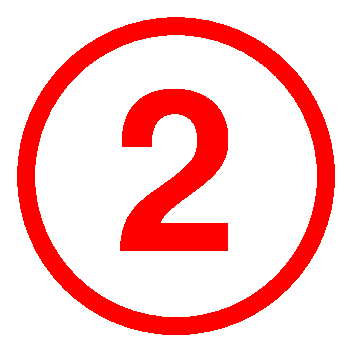
\includegraphics[scale=0.5,trim= 00 10 00 00]{../share/i/2.eps}
}

\newcommand{\TitlePicture}{%
\begin{center}%
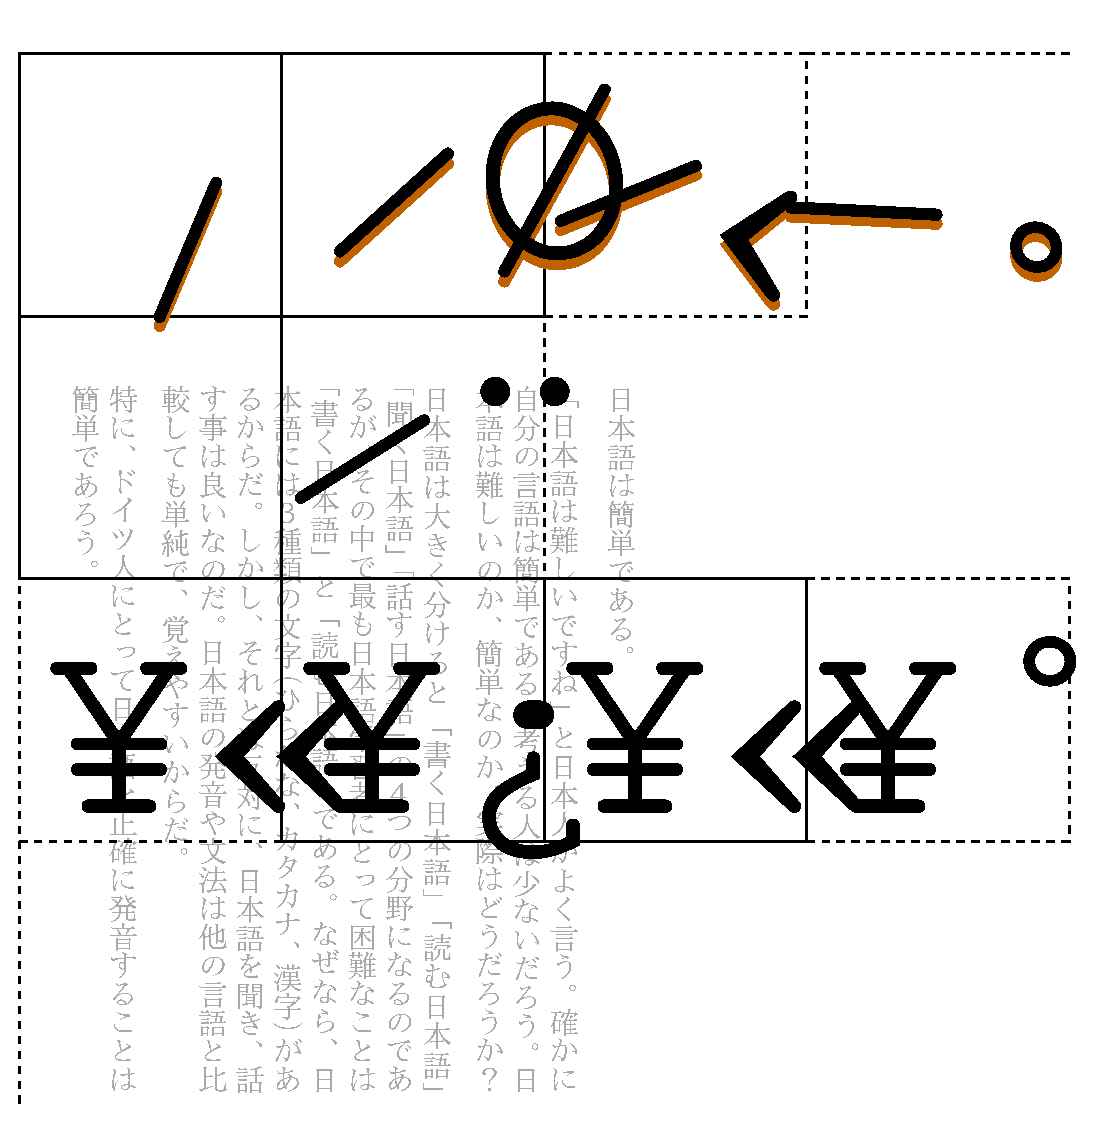
\includegraphics[scale=.5]{../share/i/kakikata-title-picture-600dpi.eps}%
\end{center}%
}%

\newcommand{\Kletter}[1]{%       l  b  r  t
\includegraphics[scale=0.95,trim=02 01 02 00]{../share/katakana/#1.pdf}
}

\newcommand{\KLETTER}[1]{%
\includegraphics[scale=2.0,trim= 00 05 00 00]{../share/katakana/#1.pdf}}

\newcommand{\Link}{ {
\includegraphics[scale=0.4,trim=00 00 01 00]{../share/i/link.pdf}} }


% PARAGRAPH COMMANDS
\newcommand{\Warn}[2]{
\begin{mdframed}[
linecolor=black!40,
outerlinewidth=1pt,
roundcorner=.5em,
innertopmargin=2ex,
innerbottommargin=.5\baselineskip,
innerrightmargin=1em,
innerleftmargin=1em,
backgroundcolor=blue!10,
%userdefinedwidth=1\textwidth,
shadow=true,
shadowsize=6,
shadowcolor=black!20,
frametitle={#1},
frametitlebackgroundcolor=red!40,
frametitlerulewidth=10pt
]

#2

\end{mdframed}
}
 % red   - additional dangerous info reg. lang
\newcommand{\Hint}[2]{
\bigskip
\relax
\begin{mdframed}[
linecolor=black!40,
outerlinewidth=1pt,
roundcorner=.5em,
innertopmargin=2ex,
innerbottommargin=.5\baselineskip,
innerrightmargin=1em,
innerleftmargin=1em,
backgroundcolor=blue!10,
%userdefinedwidth=1\textwidth,
shadow=true,
shadowsize=6,
shadowcolor=black!20,
frametitle={#1},
frametitlebackgroundcolor=blue!40,
frametitlerulewidth=10pt
]

#2

\end{mdframed}
}
 % blue  - additional important info reg. lang
% +---------------------------------------------------------------------------+
% | Info.tex                                                                  |
% |                                                                           |
% | Prints info box                                                           |
% |                                                                           |
% | Version: 0.1.1                                                            |
% |                                                                           |
% | Changes:                                                                  |
% |                                                                           |
% | 0.1.1 2020-07-23 Christian Kuelker <c@c8i.org>                            |
% |     - Add nobreak option as 3rd parameter (prevent page break)            |
% | 0.1.0 2014-08-24 Christian Kuelker <c@c8i.org>                            |
% |     - Initial release                                                     |
% |                                                                           |
% +---------------------------------------------------------------------------+


% needspace=6em:
%   https://tex.stackexchange.com/questions/201553/forbid-page-break-after-the-title-in-mdframed
%   https://kebo.pens.ac.id/CTAN/macros/latex/contrib/mdframed/mdframed-doc-en.pdf
\newcommand{\Info}[3]{
\bigskip
\relax
\begin{mdframed}[
linecolor=black!40,
outerlinewidth=1pt,
roundcorner=.5em,
innertopmargin=2ex,
innerbottommargin=.5\baselineskip,
innerrightmargin=1em,
innerleftmargin=1em,
backgroundcolor=blue!10,
%userdefinedwidth=1\textwidth,
shadow=true,
shadowsize=6,
shadowcolor=black!20,
needspace=12em,
frametitle={#1},
frametitlebackgroundcolor=green!40,
frametitlerulewidth=10pt,
nobreak=#3
]

#2

\end{mdframed}
}
 % green - additional important info
\newcommand{\Note}[2]{
\bigskip
\relax
\begin{mdframed}[
linecolor=black!40,
outerlinewidth=1pt,
roundcorner=.5em,
innertopmargin=2ex,
innerbottommargin=.5\baselineskip,
innerrightmargin=1em,
innerleftmargin=1em,
backgroundcolor=blue!10,
%userdefinedwidth=1\textwidth,
shadow=true,
shadowsize=6,
shadowcolor=black!20,
frametitle={#1},
frametitlebackgroundcolor=gray!40,
frametitlerulewidth=10pt
]

#2

\end{mdframed}
}
 % gray  - additional info
\newcommand{\Krow}[6]{
\begin{tabular}{|c|c|c|c|c|c|}\hline
\raisebox{.25\height}{
\includegraphics[scale=1.0,trim= 00 00 00 00]{../share/katakana/#1.pdf}
}
&\KLETTER{#2}&\KLETTER{#3}&\KLETTER{#4}&\KLETTER{#5}&\KLETTER{#6}\\\hline
\end{tabular}
}
 % 6 parameters
\newcommand{\Transcribe}[4]{
\begin{center}
\begin{tabular}{b{1cm}b{3cm}b{5cm}b{5cm}} 
#1 & #2 & #3 \rule[-10pt]{5cm}{.4pt} & #4 \\
\end{tabular}
\end{center}
}

\newenvironment{TranscribeEnv}{
\begin{minipage}{16cm}
\bigskip
\begin{center}
}{
\bigskip
\end{center}
\end{minipage}
}


\newcommand{\KatakanaSimpleTraining}[2]{

\bigskip

Please transcribe the following words from \textbf{#1}:

\fbox{
\begin{TranscribeEnv}
#2
\end{TranscribeEnv}
}
}


% PAGE COMMANDS
\newcommand{\KatakanaTraining}[1]{%

\bigskip Draw slowly, precise and try to make it beautiful. One line per day.

\begin{tabular}{|c|c|c|c|c|c|}\hline
\KLETTER{#1s}&\KLETTER{#1}&\KLETTER{#1g}&\KLETTER{ar}&\KLETTER{s}\\\hline
\KLETTER{s}&\KLETTER{s}&\KLETTER{s}&\KLETTER{s}&\KLETTER{s}\\\hline
\KLETTER{s}&\KLETTER{s}&\KLETTER{s}&\KLETTER{s}&\KLETTER{s}\\\hline
\end{tabular}

\bigskip Slowly from top to bottom. Precise and take care about the stroke
order. One column per hour, maximum four columns per day.

\begin{tabular}{|c|c|c|c|c|c|c|c|c|c|c|c|}\hline
\Kletter{s}&\Kletter{s}&\Kletter{s}&\Kletter{s}&\Kletter{s}&
\Kletter{s}&\Kletter{s}&\Kletter{s}&\Kletter{s}&\Kletter{#1}\\\hline
&&&&&&&&&\Kletter{#1g}\\\hline
&&&&&&&&&\Kletter{ad}\\\hline
&&&&&&&&&\Kletter{s}\\\hline
&&&&&&&&&\Kletter{s}\\\hline
\end{tabular}
\newpage

Write faster from left to right. If one character is wrong continue with slower
speed.

\begin{tabular}{|c|c|c|c|c|c|c|c|c|c|c|c|}\hline
\Kletter{#1s}&\Kletter{#1}&\Kletter{#1g}&\Kletter{ar}&\Kletter{s}&
\Kletter{s}&\Kletter{s}&\Kletter{s}&\Kletter{s}&\Kletter{s}\\\hline
&&&&&&&&&\Kletter{s}\\\hline
&&&&&&&&&\Kletter{s}\\\hline
&&&&&&&&&\Kletter{s}\\\hline
&&&&&&&&&\Kletter{s}\\\hline
&&&&&&&&&\Kletter{s}\\\hline
\end{tabular}

\bigskip Repeat the training after a week in medium pace.

\begin{tabular}{|c|c|c|c|c|c|c|c|c|c|c|c|}\hline
\Kletter{s}&\Kletter{s}&\Kletter{s}&\Kletter{s}&\Kletter{s}&
\Kletter{s}&\Kletter{s}&\Kletter{s}&\Kletter{s}&\Kletter{#1}\\\hline
&&&&&&&&&\Kletter{#1g}\\\hline
&&&&&&&&&\Kletter{ad}\\\hline
&&&&&&&&&\Kletter{s}\\\hline
&&&&&&&&&\Kletter{s}\\\hline
&&&&&&&&&\Kletter{s}\\\hline
&&&&&&&&&\Kletter{s}\\\hline
\end{tabular}
\newpage
}

\newcommand{\KatakanaHeader}[2]{%
\begin{tabular}{clr}
\raisebox{-.5\height}{\includegraphics[scale=1.0,trim= 00 00 00 00]{../share/katakana/#1t.pdf}} &
\begin{minipage}{12.5cm}
#2
\end{minipage}&
\raisebox{-.4\height}{\includegraphics[scale=2.0,trim= 00 05 00 00]{../share/katakana/#1s.pdf}} 
\\
\end{tabular}
}


% TITLE
% ===========================================================================
% TITLE
% ===========================================================================
\author{\AuthorName}
\title{ \NumberTwo\\
    The Japanese Script \\ \texttt{日本語の書き方}\\
    \bigskip \large Katakana \\ \texttt{片仮名}
}
\date{ \TitlePicture \footnotesize \jdate, v-\jversion }
\dedication{to Francesco Belletti}
\uppertitleback{ \footnotesize

Copyright \copyright~ 2000, 2001, 2002, 2003, 2004, 2005, 2006, 2013, 2014 by
\href{mailto:christian.kuelker@cipworx.org}{Christian K\"ulker}.

\medskip

See the web page 
\href{http://christian.kuelker.info/nihongo/}{http://christian.kuelker.info/nihongo/}

%” ”
%"

Permission is granted to copy, distribute and/or modify this document under the
terms of the GNU Free Documentation License (GNU-FDL), version 1.2 or any later
version published by the Free Software Foundation; with no invariant sections
except the following invariant back-cover text (see framed box below:
\textit{Back-Cover Text}).

A copy of the license is included in the section entitled ”GNU Free
Documentation License”. 

\normalsize
}
\lowertitleback{     \begin{center}
        \textbf{Back-Cover Text:}
        \begin{tabular}{|l|}\hline
            \begin{minipage}{140mm}\medskip

                The original version of this book was written by
                \textbf{Christian Külker} and is copyrighted 2000-2006,
                2013-2014 under the GNU-FDL version 1.2 or any later version
                published by the Free Software Foundation with only this
                section as invariant section. \medskip

                The version v0.1 - v0.8 of this book \textbf{日本語を書こう!}
                (German: \textit{Lasst uns Japanisch schreiben!}) was developed
                as reference and training book for the language course at the
                VHS Halle (Ravensberg) in Germany starting year 2000. It was
                published 2003, 2004 and 2006 under the GNU FDL.\medskip

                In 2014 (v0.9) the part of Katakana was made a book on its own.
                The title was changed to \textbf{日本語の書き方:片仮名}
                (English: \textit{The Japanese Script - Katakana}) and adopted
                to a self study approach.\medskip

                In 2020 (v1.0) the source code was changed to compile under
                Debian 10 Buster. Some fonts have been changed in the
                appendix.

                \medskip

                Original PDF:
                \href{https://github.com/ckuelker/nihongo/tree/master/pub/}{https://github.com/ckuelker/nihongo/tree/master/pub}

                Source Code:
                \href{https://github.com/ckuelker/nihongo/}{https://github.com/ckuelker/nihongo}

                Web site:
                \href{https://christian.kuelker.info/nihongo/}{https://christian.kuelker.info/nihongo}


                \flushright  Christian Külker, Bielefeld, \jdate, \texttt{v-\jversion}

                \medskip

            \end{minipage}\\ \hline
        \end{tabular}
    \end{center}
    \bigskip

%    \texttt{v1.0}: Appendix fonts changed.

%    \texttt{v0.9}: Initial version as Katakana only book.

%    In case you have the original book, please write to
%    \href{mailto:christian.kuelker@cipworx.org}{christian.kuelker@cipworx.org}
%    for hints, suggestions, thanks, complains.

}


% ===========================================================================
% DOCUMENT
% ===========================================================================
\begin{document}
\pagestyle{plain}
\frontmatter
\maketitle

% CONTENTS
\tableofcontents
\pagestyle{fancy}

\mainmatter

% ===========================================================================
\chapter{片仮名 - Katakana}

\Warn{Warning!}{This work is a \textbf{draft}. It is not complete and contains
errors. Please report.}

\bigskip

Katakana, written as {片仮名 【かたかな】} or {カタカナ} is the second Japanese
\hyperref[sec:Syllable]{syllable} writing system. 



% ---------------------------------------------------------------------------
\chapter{片仮名練習 - Katakana Training}

todo
\newpage

%----------------------------------------------------------------------------
\section{Katakana /a/ Row -  片仮名ア行}\label{sec:KatakanaARow}

\Krow{arow}{a}{i}{u}{e}{o}

\label{letter:a}\KLETTER{a} The 片仮名 {「ア」} derives from the
\hyperref[sec:PhoneticCharacter]{Phonetic Caracters}
(\hyperref[sec:Radical]{radical}).  A smaller version {「ァ」} is used in
combinations with other letters as {「ファ」} and is pronounced as /fa/ in
\hyperref[sec:Hepburn]{Hepburn} transcription.

\label{letter:u}\KLETTER{i} The 片仮名 {「イ」} derives from the
\hyperref[sec:PhoneticCharacter]{Phonetic Caracters} {「伊」} left element
(\hyperref[sec:Radical]{radical}).  A smaller version {「ィ」} is used in
combinations with other letters and represents a
\hyperref[sec:Diphthong]{diphthong}. 

\label{letter:u}\KLETTER{u} The 片仮名 {「ウ」} derives from the
\hyperref[sec:PhoneticCharacter]{Phonetic Caracter} {「宇」}. A smaller version
{「ゥ」} is used in combinations with other letters and represents a
\hyperref[sec:Diphthong]{diphthong} and is written as "w". Even though the
combination {「トゥ」} /tu/ exist, it is relatively new and many words do not
use it. In this cases {「ツ 」} /tsu/ is used. {「ウ」} can take
\hyperref[sec:Dakuten]{Dakuten} to form {「ヴ」} /vu/, which is relatively new
and can replace {「ブ」} /bu/. 

\Note{Note}{%

Be aware that the characters \hyperref[letter:fu]{「フ」},
\hyperref[letter:wa]{「ワ」}  and \hyperref[letter:u]{「ウ」} look very
similar.  Make sure that you spend extra training on distinguish them. 

}%


\newpage 

\label{letter:e}\KLETTER{e} The 片仮名 {「エ」} derives from the
\hyperref[sec:PhoneticCharacter]{Phonetic Caracters} {「江」} right element
(\hyperref[sec:Radical]{radical}). A smaller version {「ェ」} is used in
combinations with other letters and express \hyperref[sec:Mora]{morae} of
foreign origin. For example {「ヴェ」} as pronounced /ve/.

\label{letter:o}\KLETTER{o} The 片仮名 {「オ」} derives from the
\hyperref[sec:PhoneticCharacter]{Phonetic Caracter} {「於」}. A smaller version
{「ォ」} is used in combinations with other letters and express
\hyperref[sec:Mora]{morae} of foreign origin. For example {「フォ 」} as
pronounced /fe/.

\newpage

% ---------------------------------------------------------------------------
\subsection{/a/ - 「ア」} \label{sec:KatakanaA}

\KatakanaHeader{a}{ The Katakana {「ア」} is written with two strokes. The
first stroke starts horizontal. The second stroke is a curve with can be
attached to the first stroke in hand writing, but not at the horizontal part -
at the end of the first line.} \KatakanaTraining{a}

% ---------------------------------------------------------------------------
\subsection{/i/ - 「イ」} \label{sec:KatakanaI}

\KatakanaHeader{i}{ The Katakana {「イ」} is written with one stroke. The first
stroke is a curve from upper right to lower left. The second stroke is a
vertical line attached to the first at the top.} \KatakanaTraining{i}

% ---------------------------------------------------------------------------
\subsection{/u/ - 「ウ」} \label{sec:KatakanaU}

\KatakanaHeader{u}{The Katakana {「ウ」} is written with three strokes. The
first stroke a small vertical line. The second a small vertical line again and
the third line a horizontal line connection the two others.}
\KatakanaTraining{u}

% ---------------------------------------------------------------------------
\subsection{/e/ - 「エ」} \label{sec:KatakanaE}

\KatakanaHeader{e}{The Katakana {「エ」} is written with three strokes. It is
very geometrically consisting only out of horizontal and vertical lines
connected together.} \KatakanaTraining{e}

% ---------------------------------------------------------------------------
\subsection{/o/ - 「オ」} \label{sec:KatakanaO}

\KatakanaHeader{o}{The Katakana {「オ」} is written with three strokes. The
first line is horizontal and together with the second stroke it constructs a
perfect crossing. The third stroke beginning lies at the center of the
crossing.} \KatakanaTraining{o}

% ---------------------------------------------------------------------------
\section{/a/ Row Training - 片仮名ア行練習}
\Padding
\begin{longtable}[c]{p{2cm}p{2cm}p{3cm}p{6cm}p{2cm}}
\textit{Katakana}&\textit{Rōmaji}&\textit{Original}&\textit{Remark}&Origin\\\hline
ウエア&wuea&ware&          &English\\
エア  &ea  &air &          &English\\
エイ  &ei  &A   &the letter&English\\
\end{longtable}

\KatakanaSimpleTraining{Katakana to Romaji}{
\Transcribe{1.}{ウエア}{}{wear, ware}
\Transcribe{2.}{エア}{}{air}
\Transcribe{3.}{エイ}{}{A (the letter)}
\Transcribe{4.}{アイ}{}{I (the letter)}
\Transcribe{5.}{オウ}{}{O (the letter)}
%\Transcribe{6.}{イア}{}{ear}
}

\KatakanaSimpleTraining{Romaji to Katakana}{
\Transcribe{1.}{ea}{}{air}
\Transcribe{2.}{ai}{}{I (the letter)}
\Transcribe{3.}{ou}{}{O (the letter)}
\Transcribe{4.}{ei}{}{A (the letter)}
\Transcribe{5.}{uea}{}{wear, ware}
%\Transcribe{6.}{ia}{}{ear}
}

\newpage
\Padding
\begin{longtable}[c]{p{2cm}p{2cm}p{3cm}p{6cm}p{2cm}}
\textit{Katakana}&\textit{Rōmaji}&\textit{Original}&\textit{Remark}&Origin\\\hline
アイ  &ai  &I   &the letter&English\\
オウ  &ou  &O   &the letter&English\\
イア  &ia  &ear &          &English\\
\end{longtable}

\KatakanaSimpleTraining{English to Romaji}{
\Transcribe{1.}{ear}{}{}
\Transcribe{2.}{I (the letter)}{}{}
\Transcribe{3.}{air}{}{}
\Transcribe{4.}{O (the letter)}{}{}
\Transcribe{5.}{wear, ware}{}{}
%\Transcribe{6.}{A (the letter)}{}{}
}

\KatakanaSimpleTraining{English to Katakana}{
\Transcribe{1.}{I (the letter)}{}{}
\Transcribe{2.}{O (the letter)}{}{}
\Transcribe{3.}{air}{}{}
\Transcribe{4.}{ear}{}{}
\Transcribe{5.}{wear, ware}{}{}
%\Transcribe{6.}{A (the letter)}{}{}
}
\newpage


% ---------------------------------------------------------------------------
\section{Katakana /ka/ Row}\jsec{片仮名 カ行}\label{sec:KatakanaKaRow}

\Krow{karow}{ka}{ki}{ku}{ke}{ko}

\label{letter:ka}\KLETTER{ka} The  片仮名 {「カ」} is pronounced  /ka/ and  derives from the
\hyperref[sec:PhoneticCharacter]{Phonetic Character}s {「加」} left
\hyperref[sec:Radical]{radical}.  A \hyperref[sec:Dakuten]{濁点} version exists
and pronounced as /ga/.

%\hyperref[sec:Handakuten]{半濁点} does not exist in daily Japanese.  
% {「一ヵ所」} {【いちかしょ】} (one place)
% {「一ヶ所」} {【いちかしょ】} (one place).
% 十ヵ条(十ヶ条)


\Note{Note}{A smaller version {「ヵ」} is rare but used in combinations with
number particles.  For example in {「一ヵ月」} {【いっかげつ】} (one month) and
others.  This cases can also be written {「一ヶ月」} {【いっかげつ】} (one
month). Please see also \nameref{sec:KatakanaKe}. \Link
\href{https://ja.wikipedia.org/wiki/\%E3\%83\%B5}{ヵ} }

\label{letter:ki}\KLETTER{ki} The 片仮名 {「キ」} derives from the
\hyperref[sec:PhoneticCharacter]{Phonetic Character}s middle part of either {「機」} or
{「幾」}.  It is pronounced as /ki/.  A \hyperref[sec:Dakuten]{濁点} version
exists and pronounced as /gi/.


\label{letter:ku}\KLETTER{ku} The 片仮名 {「ク」} derives from the
\hyperref[sec:PhoneticCharacter]{Phonetic Character}s left upper part of {「久」}.  It
is pronounced as /ku/.  A \hyperref[sec:Dakuten]{濁点} version exists and
pronounced as /gu/.  A smaller version exists, but is used for the Ainu
Language.



\label{letter:ke}\KLETTER{ke} The 片仮名 {「ケ」} derives from the
\hyperref[sec:PhoneticCharacter]{Phonetic Character}s upper and left part of {「介」}.
It is pronounced as /ke/.  A \hyperref[sec:Dakuten]{濁点} version exists and
pronounced as /ge/.  The smaller version {「ヶ」} is explained in the following
note.

\newpage

\Note{Note}{ A smaller version {「ヶ」} is rare but used in combinations with
number particles.  For example in {「一ヶ月」} {【いっかげつ】} (one month) and
others.  This cases can also be written {「一ヵ月」} {【いっかげつ】} (one
month). There are cases where only {「ヶ」} can be written {七ヶ宿}
{【シチカシュク】} (Place at the south west border of the prefecture Miyagi).
In other rare cases this character can be pronounced different {「関ヶ原」}
{【せきがはら】} (Place at the south border of the Gifu prefecture, known by
the battle at 1600.). Please see also \nameref{sec:KatakanaKa}. \Link
\href{https://ja.wikipedia.org/wiki/\%E3\%83\%B5}{ヵ} }

\label{letter:ko}\KLETTER{ko} The 片仮名 {「コ」} derives from the
\hyperref[sec:PhoneticCharacter]{Phonetic Character}s upper part of {「己」}.  It is
pronounced as /ko/.  A \hyperref[sec:Dakuten]{濁点} version exists and
pronounced as /go/.



\newpage

% ---------------------------------------------------------------------------
\subsection{/ka/}\jsubsec{「カ」} \label{sec:KatakanaKa}

\KatakanaHeader{ka}{ /ka/ is written with 2 strokes. Basically the same way as
the Hiragana {「か」} it looks like a squarish version, but without the last
stroke. The hook at the second stroke is less significant or important.  }
\KatakanaTraining{ka}

% ---------------------------------------------------------------------------
\subsection{/ki/}\jsubsec{「キ」} \label{sec:KatakanaKi}

\KatakanaHeader{ki}{ The shape alignment of the 「キ」character is not straight
towards its environment. However the junctions are more or less 90 degrees.  }
\KatakanaTraining{ki}

% ---------------------------------------------------------------------------
\subsection{/ku/}\jsubsec{「ク」} \label{sec:KatakanaKu}
% ---------------------------------------------------------------------------

\KatakanaHeader{ku}{ The first stroke is similar the stroke of {「ケ 」} is a
curve. While the second stroke start aligned and straight. }
\KatakanaTraining{ku}

% ---------------------------------------------------------------------------
\subsection{/ke/}\jsubsec{「ケ」} \label{sec:KatakanaKe}

\KatakanaHeader{ke}{ The {「ケ 」} is written with 3 strokes and the first
stroke is similar to the {「ク」}. The second stroke is aligned and straight.
While the last stroke is a curve.  } \KatakanaTraining{ke}

% ---------------------------------------------------------------------------
\subsection{/ko/}\jsubsec{「コ」} \label{sec:KatakanaKo}

\KatakanaHeader{ko}{ This character is almost a geometric figure composed out
of two strokes. However unless in European languages this are only 2 strokes
and not 3. The first stroke is the longest one and done similar with all
{漢字}. } \KatakanaTraining{ko}

% ---------------------------------------------------------------------------
\subsection{/ka/ Row Training}\jsubsec{片仮名カ行練習}

\Padding
\begin{longtable}[c]{p{2cm}p{1.5cm}p{1.5cm}p{3cm}p{7cm}}
\textit{Katakana}&\textit{Rōmaji}&\textit{Original}&\textit{Remark}&Origin\\\hline
カキ  &kaki &kaki &柿 persimon&Japanese\\
ケア  &kea  &care &          &English\\
ケイ  &kei  &K    &the letter&English\\
\end{longtable}

\KatakanaSimpleTraining{Katakana to Rōmaji}{
\Transcribe{1.}{カキ}{}{persimmon}
\Transcribe{2.}{ココア}{}{cocoa}
\Transcribe{3.}{ケア}{}{care}
\Transcribe{4.}{コア}{}{core}
\Transcribe{5.}{ケーキ}{}{cake}
%\Transcribe{6.}{ケイ}{}{K (the letter)}
}

\KatakanaSimpleTraining{Rōmaji to Katakana}{
\Transcribe{1.}{kokoa}{}{cocoa}
\Transcribe{2.}{k$\overline{\mbox{e}}$ki}{}{cake}
\Transcribe{3.}{kea}{}{care}
\Transcribe{4.}{koa}{}{core}
\Transcribe{5.}{kaki}{}{persimmon}
%\Transcribe{6.}{kei}{}{K (the letter)}
}

\newpage

\Padding
%\begin{longtable}[c]{p{2cm}p{2cm}p{3cm}p{6cm}p{2cm}}
\begin{longtable}[c]{p{2cm}p{2.0cm}p{3.5cm}p{4cm}p{2.5cm}}
\textit{Katakana}&\textit{Rōmaji}&\textit{Original}&\textit{Remark}&Origin\\\hline
コア  &koa  &core &          &English\\
ココア&kokoa&cocoa& hot chocolate &English, from metathesis of Spanish cacao, from Nahuatl cacahuatl\\
ケーキ&kēki &cake &          &English\\
\end{longtable}


\KatakanaSimpleTraining{English to Rōmaji}{
\Transcribe{1.}{persimon}{}{}
\Transcribe{2.}{cocoa}{}{}
\Transcribe{3.}{care}{}{}
\Transcribe{4.}{core}{}{}
\Transcribe{5.}{K (the letter)}{}{}
%\Transcribe{6.}{cake}{}{}
}

\KatakanaSimpleTraining{English to Katakana}{
\Transcribe{1.}{cocoa}{}{}
\Transcribe{2.}{cake}{}{}
\Transcribe{3.}{care}{}{}
\Transcribe{4.}{persimon}{}{}
\Transcribe{5.}{K (the letter)}{}{}
%\Transcribe{6.}{core}{}{}
}

\newpage


\begin{tabular}{|c|c|c|c|c|c|}\hline
 & a & i & u & e & o \\\hline
-&\Kletter{a}&\Kletter{i}&\Kletter{u}&\Kletter{e}&\Kletter{o}\\\hline
\end{tabular}

% ===========================================================================
\chapter{専門用語 - Terminology}

% ---------------------------------------------------------------------------
\section{Man'yōgana}\jsec{万葉仮名}
% [o] LABEL
\label{sec:Manyogana}
\label{sec:Manyoshu}
% [o] INDEX
\ifor{Man'yōgana}{万葉仮名}{まんようがな}{Man'yōgana}
\ifor{Man'yōshu}{万葉集}{まんようしゅう}{Man'yōshu}
\ifor{mora}{モーラ}{もーら}{Mora}
\ifor{Kanji}{漢字}{かんじ}{Kanji}
\ifor{Katakana}{片仮名}{かたかな}{Katakana}

The development of distinct Japanese writing begun 600 AD by writers and
scholars reducing some Chinese characters to its bare phonetic value. The
meaning of this characters where ignored. Around 760 a collection of Japanese
poetry was published, the \Link
\href{http://en.wikipedia.org/wiki/Man%27y%C5%8Dsh%C5%AB}{万葉集
【まんようしゅう】}, in which Chinese characters where uses as phonetic
letters. In regard to \textit{Man'yōshu} {万葉集} {【まんようしゅう】} the
characters are named {万葉仮名} {【まんようがな】}

The origin of the \textbf{Man'yōgana} script in poetry and art lead to some
problems in the understanding for the reader. Since the usage of phonetic
Chinese characters where mixed with regular Chinese characters and the
reasoning about which character to use was more form and shape aesthetic then
pragmatic, the meaning was difficult to grasp.

However the royal household or other scholars did not see a necessity to change
the status quo, because the high aim was to write poetry and other texts in
Chinese and \textbf{Man'yōgana} was considered appropriate only for notes,
diaries and love letters.

\Note{Note}{\footnotesize By the end of the 8th Century 970
\hyperref[sec:Kanji]{{漢字} {【かんじ】}} where used to pronounce the 90
\hyperref[sec:Mora]{morae}. This directly shows that there was no bijective map
between sound and character. For |ka| for example the following
\textbf{Man'yōgana} can be used {「可」}, {「何」}, {「加」}, {「架」},
{「香」}, {「蚊」}, {「迦」}. }

\newpage

The number of \textbf{Man'yōgana} from which \hyperref[sec:Katakana]{Katakana}
likely derived is smaller.  


\Hint{Man'yōgana used for creation of {片仮名} {【かたかな】}}{
\begin{center}
\begin{tabular}{|c||c|c|c|c|c|}\hline
 & a& i  & u  & e& o\\\hline\hline
-&阿&伊  &宇  &江&於\\\hline
k&加&機幾&久  &介&己\\\hline
s&散&之  &須  &世&曽\\\hline
t&多&千  &州川&天&止\\\hline
n&奈&仁  &奴  &祢&乃\\\hline
h&八&比  &不  &部&保\\\hline
m&末&三  &牟  &女&毛\\\hline
y&也&    &由  &  &與\\\hline
r&良&利  &流  &礼&呂\\\hline
w&和&井  &    &恵&乎\\\hline
*&尓&    &    &  &  \\\hline
\end{tabular}
\end{center}
}

The scientific term \textbf{Man'yōgana} is used by Western and Japanese
scientists. However it is not without critique. The term \textbf{Man'yōgana}
might lead to the illusion that it was a defined set of characters in use for
transcribing Chinese or writing Japanese texts or the second illusion that one
sound is represented by only  one \textbf{Man'yōgana}. Both is not true. First,
all Chinese Characters could in principle be used as \textbf{Man'yōgana} (and
therefore the term is basically useless). Actually the reason to chose one
character was sometimes just because out of aesthetic reasons, the shape or
some additional meaning. And second, normally many different
\textbf{Man'yōgana} (Chinese characters) where used for the same pronunciation
in the same text.  Making it efficient or easy was not the target of the
scholars using this kind of \hyperref[sec:PhoneticCharacter]{phonetic
characters} at that time.


\Link \href{http://en.wikipedia.org/wiki/Manyogana}{Man'yōgana}
\Link \href{http://en.wikipedia.org/wiki/Man%27y%C5%8Dsh%C5%AB}{万葉集}

 % label sec:Manyogana

% ---------------------------------------------------------------------------
\section{Hepburn System}\jsec{ヘボン式}
%[o] LABEL
\label{sec:Hepburn}
\label{sec:HepburnSystem}
\label{sec:OlderHepburnSystem}
\label{sec:NewerHepburnSystem}
% [o] INDEX
\ifor{Hepburn System}{ヘボン式}{へぼんしき}{Hepburn System}
\ifor{older Hepburn System}{標準ヘボン式ローマ字}{ひょうじゅん・へぼん・ろまあじ}{altes Hepburn System}
\ifor{newer Hepburn System}{修正ヘボン式ローマ字}{しゅうせい・へぼんしき・ろうまじ}{neueres Hepburn System}
\ithree{James Curtis Hepburn}{James Curtis Hepburn}{James Curtis Hepburn}

\begin{tabular}{lr}
\begin{minipage}{10.5cm}

The { ヘボン式} {【へぼんしき】} is one of the two most important transcription
systems for Japanese written \hyperref[sec:Mora]{morae} based language. The
{ヘボン式} is most used system worldwide and in Japan.

The word {ヘボン} (hebon) is an old writing of the name \textbf{Hepburn}, a US
American physician, translator, educator and lay Christian missionary, who used
it his first Japanese English Dictionary (3rd ed.) in 1867.

There are manly two different variants. The older {標準ヘボン式ローマ字}
{【ひょうじゅん・へぼん・ろまあじ】} variant, which is used for signs at train
stations. And the new variant the {修正ヘボン式ローマ字}
{【しゅうせい・へぼんしき・ろうまじ】} which is used as a revised system since
1954 in Kenkyusha dictionaries. Most western scientists are using this system.
This system is also used in this book.

\Link \href{http://en.wikipedia.org/wiki/James_Curtis_Hepburn}{Hepburn}

\end{minipage}
&
\raisebox{-.47\height}{
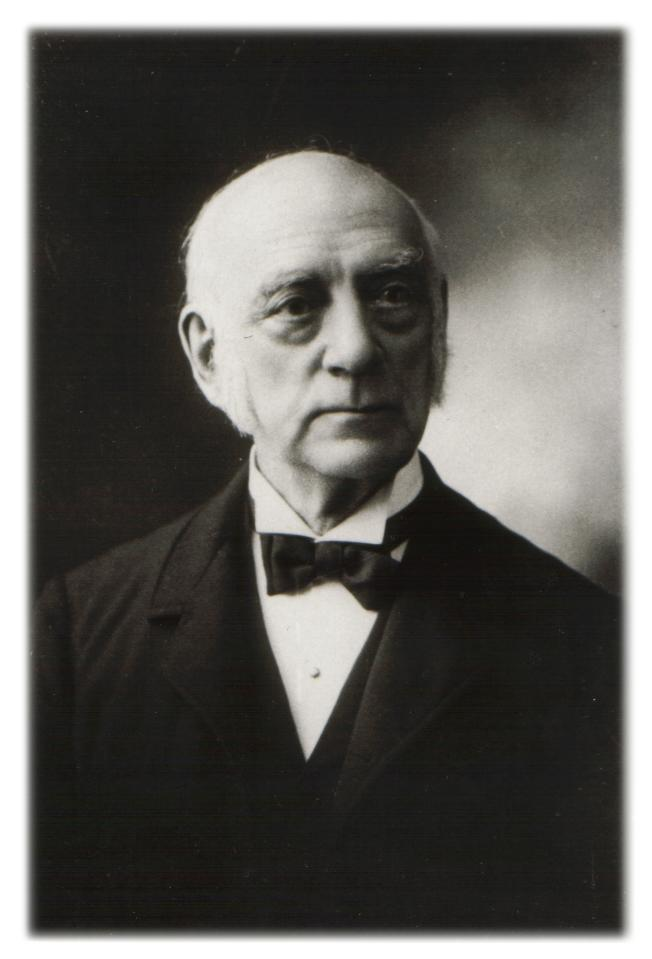
\includegraphics[scale=0.5,trim= 00 00 00 00]{../share/ei/James_Curtis_Hepburn.jpg}}
\\
\end{tabular}


 % label sec:Hepburn

\section{Kunrei System}\jsec{訓令式ローマ字} 
% [o] LABEL
\label{sec:Kunrei}
\label{sec:KunreiSystem}
\label{sec:JapanSystemLatinLetters}
% [o] INDEX
\ifor{Kunrei system}{訓令式ローマ字}{くんれいろうまじ}{Kunrei System}
\ifor{Japan system Latin letters}{日本式ローマ字}{にほんしきろうまじ}{Lateinische Buchstaben des Japanischen Systems}
\ifor{Katakana}{片仮名}{かたかな}{Katakana}
\ifor{Gojūonzu}{五十音図}{ごじゅうおんず}{50 Laute Tafel}
\begin{tabular}{lr}
\begin{minipage}{9.6cm}

The modern \textbf{Kunrei} System {訓令式ローマ字} {【くんれいろうまじ】}  is
the official writing system of Japan. It was confirmed in 1994 by the Cabinet
and is available as ISO 3602:1989. The \textbf{Kunrei} System predecessor was
introduced 1985 by Dr. Aikitsu Tanakadatei ({田中舘愛橘}) as {日本式ローマ字}
{【にほんしきろうまじ】} (Nihon-/Nipponshikiromaji) and tries a more
systematical approach to map \hyperref[sec:Hiragana]{Hiragana} and
\hyperref[sec:Katakana]{Katakana} to equal Roman letters. The {五十音図}
{【ごじゅうおんず】} in the {訓令式ローマ字} is as follows:

\Link \href{http://en.wikipedia.org/wiki/Tanakadate_Aikitsu}{Tanakadate}

\end{minipage}
&
\raisebox{-.5\height}{
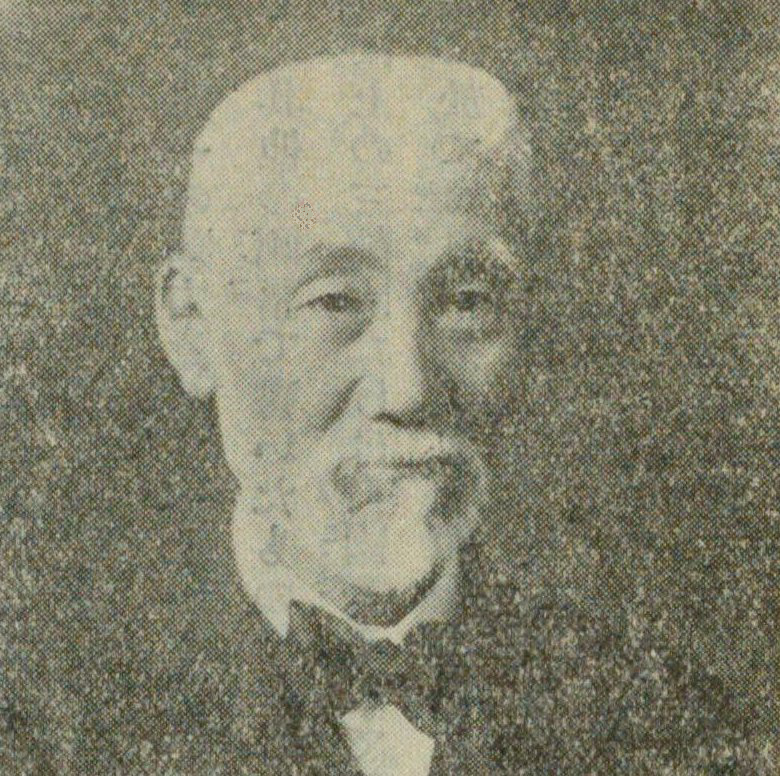
\includegraphics[scale=0.25,trim= 00 00 00 00]{../share/ei/Aikitsu_Tanakadate_r.jpg}}
\\
\end{tabular}


\Info{訓令式ローマ字 - Kunrei System}{
\begin{center}
\begin{tabular}{|c|c|c|c|c|}\hline
   a & i& u& e& o\\\hline
   ka&ki&ku&ke&ko\\\hline
   sa&si&su&se&so\\\hline
   ta&ti&tu&te&to\\\hline
   na&ni&nu&ne&no\\\hline
   ha&hi&hu&he&ho\\\hline
   ma&mi&mu&me&mo\\\hline
   ya&  &yu&  &yo\\\hline
   ra&ri&ru&re&ro\\\hline
   wa&  &  &  & o\\\hline
     &  &  &  & n\\\hline
\end{tabular}
\end{center}
}{true}

Even tough the system is official, many entities (like the train system) are
not using it. They use the Hepburn System.

The {訓令式ローマ字} is not part of this book. Please see \nameref{sec:Hepburn}
(on page \pageref{sec:Hepburn}) for the system in use.
 % label sec:Kunrei

% ---------------------------------------------------------------------------
\section{Diphthong}\jsec{二重母音} \label{sec:Diphthong}
\ithree{diphthong}{二重母音}{Diphthong}
\ithree{diphthong}{にじゅうぼいん}{Diphthong}
\ithree{syllable}{音節}{Silbe}
\ija{「アエ」}
\ija{「アイ」}
\ija{「アウ」}
\ija{「アオ」}
\ija{「ウエ」}
\ija{「ウイ」}
\ija{「オエ」}
\ija{「オイ」}
\ija{「オウ」}

A \textbf{diphthong} {二重母音} {【にじゅうぼいん】} is a sound that is
constructed from two different sounds that glide into each other while
pronouncing and form a \hyperref[sec:Syllable]{syllable}. A \textbf{diphthong}
is made out of vocals.  Examples for a \textbf{diphthong} in Japanese are {姪}
|me.i| and {甥} |o.i|.  Also  {「アエ」}, {「アイ」}, {「アウ」},
{「アオ」}、{「ウエ」}, {「ウイ」}, {「オエ」}, {「オイ」} or {「オウ」} are
likely to appear as a \textbf{diphthong} in normal conversation in Japanese.
However, they becomes vowel connections when it is pronounced slowly and it is
treated as two vowels in the consciousness of the Japanese speaker.
 % label: sec:Diphthong

% ---------------------------------------------------------------------------
\section{Mora - モーラ} \label{sec:Mora}

The concept of "mora"  (plural morae or moras; often symbolized μ) is used in
the science of linguistics. It describes a joint unit in pronunciation
(phonology) that constructs a syllable. The definition of a mora can vary.  In
Japanese the detection of morae is comparably simple. The world
{「チョコレート」} for example consist out of the following 5 morae
{「チョ」},{「コ」},{「レ」},{「ー」} and {「ト」} while it consist only out of
four \hyperref[sec:Syllable]{syllables} {(\hyperref[sec:Syllable]{音節}
【おんせつ】)}.

 % label sec:Mora

% ---------------------------------------------------------------------------
\section{Syllable - 音節} \label{sec:Syllable}

A \textbf{syllable} {音節}  {【おんせつ】}  is a phonetic building block for
words. It influences the rhythm of a spoken language. In Western languages a
\textbf{syllable} is made out of one or more letters. In Japanese it is often
one character (of \hyperref[sec:Kana]{Kana}), but not always. For a better
understanding of the Japanese it is important to understand the concept of
\hyperref[sec:Mora]{mora}.

\Link \href{http://en.wikipedia.org/wiki/Syllable}{Syllable}
\Link \href{http://ja.wikipedia.org/wiki/%E9%9F%B3%E7%AF%80}{音節}

 % label sec:Syllable

% ---------------------------------------------------------------------------
\section{Dakuten}\jsec{濁点} \label{sec:Dakuten}
\ithree{diacritic sign}{濁点}{Diakritisches Zeichen}
\ithree{diacritic sign}{だくてん}{Nigorierungszeichen}
\ithree{Umlaut}{ウムラウト}{Umlaut}
\ithree{syllable}{音節}{Silbe}

The \textbf{Dakuten} - Japanese {濁点} {【だくてん】} - is a diacritic sign.
Similar to the German Umlaut.  The {濁点} is referenced colloquial as {点々}
{【てんてん】}.  It us used to in {仮名} \hyperref[sec:Syllable]{syllabaries}
to mark a consonant to be pronounced voiced. Two strokes {「゙」} are used near
the Katakana letter.  For other {濁点}, please see \nameref{sec:Iteration} on
page \pageref{sec:Iteration}.

 % label sec:Dakuten

% ---------------------------------------------------------------------------
\section{Handakuten - 半濁点} \label{sec:Handakuten}

In Japanese two different {濁点} {【だくてん】} are used. The {濁点}  and  the
{半濁点} {【はんだくてん】} has the marker of a little circle {「゚」} and is
therefore colloquially described as {丸} {【まる】} and indicates when the
pronunciation shifts from |h| to |p|.

 % label sec:Handakuten

% ---------------------------------------------------------------------------
\section{Katakana Iteration Marks} \label{sec:Iteration}

As with {漢字} {【かんじ】} also {片仮名} has a iteration mark.  「ヽ」 and its
{濁点} {【だくてん】} form {「ヾ」}. This can only be
found in rare cases. For example the personal name Misuzu 【みすゞ】might
contain this character. And since the difference between the second last
and the last mora is only a change in pronunciation the {濁点} is added.

In vertical writing exist another iteration marker {くの字点} {【くのじてん】}
which consist out of two characters {「〳」+「〵」} and the {濁点} form
is {「〴」+「〵」}

 % label sec:Iteration

% ---------------------------------------------------------------------------
\section{Radical}\jsec{部首}
% [o] LABEL
\label{sec:Radical}
% [o]  INDEX
\ifor{radical}{部首}{ぶしゅ}{Radikal}
\ifor{Kanji}{漢字}{かんじ}{Kanji}

A \textbf{radical} {部首} {【ぶしゅ】} is a root particle or character of a
Sino-Japanese character {漢字} {【かんじ】}. It is the most significant part of
a Sino-Japanese character. The concept was developed in China for Chinese
characters and is today known under the same name {部首} (pinyin: bùshǒu).

There is no general definition what a \textbf{radical} is or how many are
existing and it can vary a lot. The author of a dictionary has the power to
defined what a \textbf{radical} is and how much there will be in that
dictionary.

In more traditional Chinese or Japanese dictionaries a number of 214 or 244
\textbf{radicals} is quite common. However some modern approaches like the
\Link \href{http://www.hadamitzky.de/english/works_books.htm#KD}{\textit{The
Kanji Dictionary} of Marc Spahn and Wolfgang Hadamitzky from 1996} a totally
different number of 79 can be found.

\Note{Note}{\footnotesize Before buying a \hyperref[sec:Kanji]{Kanji}
dictionary, make sure that the \textbf{radical} system used suits your taste.
Sometimes it can be observed that Japanese dictionaries are stricter in the
definition of a \textbf{radical} because a given \hyperref[sec:Kanji]{Kanji}
can only be retrieved via exactly \textit{one} \textbf{radical}. While in many
Chinese dictionaries \textit{every} \textbf{radical} of a Chinese character can
be used to find it. The Japanese approach is of course good in terms of
systematic and didactic for learners, however it can take significant longer to
look up a character by \textbf{radical}.  }

 % label sec:Radical

% ===========================================================================
% END
% ===========================================================================
\end{document}
